\section{Practice with linear filters }\label{P3}

As part of this segment, a variety of linear filters are applied to the image in order to see the effects that each filter has on the picture. It is clear from looking at Figure 10 that the first filter does not alter the image in any way because it merely adds the intensity of the central pixel and gives the neighboring pixels no weight at all. When we talk about the filters in image (b), we are referring to those filters that alter the position of the image and shift it in either the horizontal or vertical direction. The value of the central pixel is changed to the value of a nearby filter when this filter is applied. Image (c) and image (d) demonstrate the effect that a sharpening filter has on an image. It is possible to improve the edges and certain details in a picture by using a sharpening filter, which is also often known as an edge-enhancement filter. This filter is used to make the edges and details appear more prominent. Sometimes it is used to improve the quality of a picture in some way by increasing the contrast at the boundaries of regions of differing pixel intensity values. This is usually done in order to improve the overall image quality. By using this filter, dark sections will appear darker, while light regions will appear lighter at the edges of the image. Because an excessive amount of sharpening (image (d) of Figure 10) can cause an image to appear unnatural and can result in the loss of certain critical information, it is essential to apply sharpening filters in the correct manner during the editing process.

\begin{figure}[h]
    \centering
    \begin{subfigure}{0.4\textwidth}
        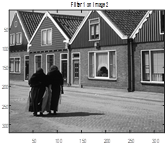
\includegraphics[width=\textwidth]{Resources/F10-a.png}
        \caption{}
        \label{fig:first}
    \end{subfigure}
    \hfill
    \begin{subfigure}{0.4\textwidth}
        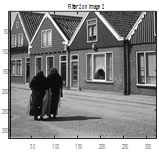
\includegraphics[width=\textwidth]{Resources/F10-b.png}
        \caption{}
        \label{fig:Second}
    \end{subfigure}
    \vfill
    \begin{subfigure}{0.4\textwidth}
        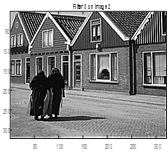
\includegraphics[width=\textwidth]{Resources/F10-c.png}
        \caption{}
        \label{fig:first}
    \end{subfigure}
    \hfill
    \begin{subfigure}{0.4\textwidth}
        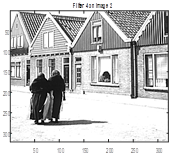
\includegraphics[width=\textwidth]{Resources/F10-d.png}
        \caption{}
        \label{fig:Second}
    \end{subfigure}
    \caption{Using different linear filters on images}
    \label{fig:ApplyingFilters}
\end{figure}
